\documentclass[]{article}
\usepackage{lmodern}
\usepackage{amssymb,amsmath}
\usepackage{ifxetex,ifluatex}
\usepackage{fixltx2e} % provides \textsubscript
\ifnum 0\ifxetex 1\fi\ifluatex 1\fi=0 % if pdftex
  \usepackage[T1]{fontenc}
  \usepackage[utf8]{inputenc}
\else % if luatex or xelatex
  \ifxetex
    \usepackage{mathspec}
  \else
    \usepackage{fontspec}
  \fi
  \defaultfontfeatures{Ligatures=TeX,Scale=MatchLowercase}
\fi
% use upquote if available, for straight quotes in verbatim environments
\IfFileExists{upquote.sty}{\usepackage{upquote}}{}
% use microtype if available
\IfFileExists{microtype.sty}{%
\usepackage{microtype}
\UseMicrotypeSet[protrusion]{basicmath} % disable protrusion for tt fonts
}{}
\usepackage[margin=1in]{geometry}
\usepackage{hyperref}
\hypersetup{unicode=true,
            pdftitle={Detecting marine heatwaves with sub-optimal data},
            pdfauthor={Robert W. Schlegel(1,2), Eric C. J. Oliver(1), Alistair J. Hobday(3), Albertus J. Smit(2)},
            pdfborder={0 0 0},
            breaklinks=true}
\urlstyle{same}  % don't use monospace font for urls
\usepackage{graphicx,grffile}
\makeatletter
\def\maxwidth{\ifdim\Gin@nat@width>\linewidth\linewidth\else\Gin@nat@width\fi}
\def\maxheight{\ifdim\Gin@nat@height>\textheight\textheight\else\Gin@nat@height\fi}
\makeatother
% Scale images if necessary, so that they will not overflow the page
% margins by default, and it is still possible to overwrite the defaults
% using explicit options in \includegraphics[width, height, ...]{}
\setkeys{Gin}{width=\maxwidth,height=\maxheight,keepaspectratio}
\IfFileExists{parskip.sty}{%
\usepackage{parskip}
}{% else
\setlength{\parindent}{0pt}
\setlength{\parskip}{6pt plus 2pt minus 1pt}
}
\setlength{\emergencystretch}{3em}  % prevent overfull lines
\providecommand{\tightlist}{%
  \setlength{\itemsep}{0pt}\setlength{\parskip}{0pt}}
\setcounter{secnumdepth}{0}
% Redefines (sub)paragraphs to behave more like sections
\ifx\paragraph\undefined\else
\let\oldparagraph\paragraph
\renewcommand{\paragraph}[1]{\oldparagraph{#1}\mbox{}}
\fi
\ifx\subparagraph\undefined\else
\let\oldsubparagraph\subparagraph
\renewcommand{\subparagraph}[1]{\oldsubparagraph{#1}\mbox{}}
\fi

%%% Use protect on footnotes to avoid problems with footnotes in titles
\let\rmarkdownfootnote\footnote%
\def\footnote{\protect\rmarkdownfootnote}

%%% Change title format to be more compact
\usepackage{titling}

% Create subtitle command for use in maketitle
\providecommand{\subtitle}[1]{
  \posttitle{
    \begin{center}\large#1\end{center}
    }
}

\setlength{\droptitle}{-2em}

  \title{Detecting marine heatwaves with sub-optimal data}
    \pretitle{\vspace{\droptitle}\centering\huge}
  \posttitle{\par}
    \author{Robert W. Schlegel(1,2), Eric C. J. Oliver(1), Alistair J. Hobday(3),
Albertus J. Smit(2)}
    \preauthor{\centering\large\emph}
  \postauthor{\par}
      \predate{\centering\large\emph}
  \postdate{\par}
    \date{April 30th, 2018}


\begin{document}
\maketitle

1: Department of Oceanography, Dalhousie University, Halifax, Nova
Scotia, Canada 2: Department of Biodiversity and Conservation Biology,
University of the Western Cape, Bellville, South Africa 3: CSIRO Oceans
and Atmosphere, Hobart, Tasmania, 7000, Australia

\section{Abstract}\label{abstract}

Marine heatwaves (MHWs), or prolonged periods of anomalously warm sea
water temperature, have been increasing in duration and intensity
globally for decades. However, there are many coastal, oceanic, and
polar regions where our ability to detect MHWs is uncertain due to the
unavailability of high-quality data. Here we investigate the effect that
short time series length, missing data, or linear decadal temperature
trends may have on the detection of MHWs. We show that MHWs detected in
time series as short as 10 years did not have durations or intensities
significantly different from events detected in the standard length 30
year time series, but the accurate identification of temperature
thresholds could be impaired when fewer than 15 years of data were used.
We also show that the output of the MHW algorithm for time series
missing less than 20\% data did not differ appreciably, and that this
could be increased to 40\% when gaps were filled with linear
interpolation. Linear decadal trends of 0.05 -- 0.15°C/dec could lead to
inaccurate creation of seasonal climatologies, but this did not impact
accurate MHW detection. The percentage of missing data in a time series
was determined to have the largest effect on the detection of MHWs, but
was also the easiest to correct for. Time series length had less of an
effect on MHW detection, but was more difficult to correct for. We
provide suggestions for best practices to improve the accuracy of MHW
detection with sub-optimal time series on a global scale and specific
case studies of three notable MHWs from the literature.\\

<<<<<<< HEAD
\hypertarget{introduction}{%
\section{Introduction}\label{introduction}}
=======
\section{Introduction}\label{introduction}
>>>>>>> 59f30a2abb8f68303f0eba570fc6e00bb2250a7f

The idea of locally warm seawater being problematic is not a novel
concept. We have known for decades that seemingly transient warm water
occurrences in the ocean could result in major impacts (e.g. Baumgartner
1992, Salinger et al. (2016)). The study of the effects of anomalously
warm seawater temperatures began in earnest in the early 1980's when
research into the ENSO phenomenon began (e.g. Philander 1983). After the
1980's, researchers began noticing that warm water events were becoming
more frequent and problematic, but it wasn't until 2018 that this was
demonstrated with global observations (Oliver et al. 2018).

In order to quantify the increased occurrence and severity of these
events it was necessary to develop a methodology that would be
inter-comparable for the entire planet. This was accomplished in 2016
after the International Working Group on Marine Heatwaves
(marineheatwaves.org) initiated a series of workshops to address this
issue (Hobday et al. 2016). This definition for anomalously warm
seawater events, known as marine heatwaves (MHWs), has seen wide-spread
and rapid adoption due to ease of use and applicability to any part of
the globe. One problem with this algorithm that has not yet been
addressed is the assumption that a researcher has access to the highest
quality data available when detecting MHWs. In the context of MHW
detection `high quality' is a daily time series with no missing data
that is at least 30 years in length. To avoid contention on the use of
the word `quality', time series that meet the aforementioned standard
are referred to here as `optimal', whereas those that do not meet some
part of the standard are referred to as `sub-optimal'.

Most remotely-sensed data, and more recently output from ocean models
and reanalyses, consist of over 30 years of data and utilise statistical
techniques to fill gaps in the time series from a number of
environmental and technical sources. This means that these data are
considered optimal for MHW detection however, they still have issues
(e.g.~land bleed and incorrect data flagging) and so it may be
recommended that researchers utilise sub-optimal data when possible,
such as sporadically collected \emph{in situ} time series. Coastal areas
are often poorly sampled yet are the most susceptible to the impacts of
MHWs (e.g. Smale et al. 2019) so it is necessary to address the issues
that using these data may have on the detection of MHWs.

This paper seeks to understand the limitation of using sub-optimal data
for the detection of MHWs. Of primary interest are three key challenges:
1) The use of short time series, 2) the use of time series with missing
data, 3) the use of time series in areas with large long-term
temperature trends. We will use a combination of reference time series
from specific locations and global data to address these issues. The
effects of the three sub-optimal data challenges on the detection of
MHWs are quantified in order to provide researchers with the level of
confidence they may express in their results. Where possible, best
practices for the correction of these issues are detailed.

\section{Defining marine heatwaves}\label{defining-marine-heatwaves}

The definition used in this paper for a MHW is ``a prolonged discrete
anomalously warm water event that can be described by its duration,
intensity, rate of evolution, and spatial extent.'' (Hobday et al.
2016). This qualitative definition is quantified with an algorithm that
calculates a suite of metrics. These metrics may then be used to
characterise MHWs and to effectively compare them against known
ecological/financial impacts. The calculation of these metrics is made
possible by first determining the mean and 90th percentile temperature
for each of the 366 calendar day-of-year (doy) in a time series. The
mean doy temperatures, which also represent the seasonal signal in the
time series, provide the expected baseline temperature whose daily
exceedance is used to calculate the intensity of MHWs. The 90th
percentile doy temperatures serve as the threshold that must be exceeded
for 5 or more consecutive days for the anomalously warm temperatures to
be classified as a MHW and for the calculation of the MHW metrics to
begin.

In this paper we will focus on the two metrics that most succinctly
summarise a MHW. The first metric, \emph{duration (days)}, is defined as
the number of days that the temperature remains at or above the 90th
percentile threshold without dipping below it for more than 2
consecutive days. The duration of an event is the best single
measurement of the chronic stress that a MHW may inflict upon a target
species or ecosystem. The second metric, \emph{maximum intensity (°C)},
is the single warmest day during the event and is calculated by
subtracting the mean doy temperature on that day from the recorded
temperature. This metric is the best single representation of acute
stress. There are many other MHW metrics and the full explanation for
them may be found in Table 2 of Hobday et al. (2016).

Hobday et al. (2018) extended the MHW definition to include a
categorisation scheme based on the intensity of an event. These
categories were: I Moderate, II Strong, III Severe, and IV Extreme. The
category of an event is determined by how many times the maximum
intensity of the MHW is a multiple of the difference between the mean
and 90th percentile doy temperatures (Figure 1). For example, if the
difference between the mean and 90th percentile doy temperatures on the
warmest day of a MHW 1.5°C, and the temperature recorded on that warmest
day was 3°C warmer than the mean doy temperature for that day, this
would be considered a category II (Strong) MHW. Were the maximum
temperature recorded at 4.5°C, this would then be classified as a
category III Severe MHW. To provide a more robust qualification of a
MHW, the categories are also calculated for each day of a MHW to provide
a proportion of the days during which the event was within each of the
categories.

An additional advantage in the use of the Hobday et al. (2016) and
Hobday et al. (2018) approach is that it has been developed for python
(\url{https://github.com/ecjoliver/marineHeatWaves}), R (Schlegel and
Smit 2018), and MATLAB (Zhao and Marin 2019). For this analysis we
compared the R and python default outputs, assessed how changing the
arguments affected the results, and compared the other functionality
provided between the two languages. While some style differences exist
between the added functionality of the languages, the core climatology
outputs are identical to within \textless{} 0.001 °C per day-of-year
(doy). An independent analysis of the Python and MATLAB results also
confirmed that they were functionally identical (pers. com. Zijie Zhao;
MATLAB distribution author).

\begin{figure}
\centering
\includegraphics{../LaTeX/fig_1.png}
\caption{Figure 1: The focus marine heatwaves (MHWs) from the three
reference time series A) Western Australia, B) Northwest Atlantic, and
C) Mediterranean. The various thresholds for the different MHW
categories are shown as grey dotted lines and the proportions of the MHW
within each category are filled with the corresponding colours seen in
the legend at the top of the figure. Each panel is centred around the
peak date of the focus MHW. The peak date is further highlighted by a
dark green vertical segment. The beginning and end of each event are
demarcated with light green vertical segments.}
\end{figure}

<<<<<<< HEAD
\hypertarget{what-are-optimal-data-for-detecting-marine-heatwaves}{%
=======
>>>>>>> 59f30a2abb8f68303f0eba570fc6e00bb2250a7f
\section{What are optimal data for detecting marine
heatwaves?}\label{what-are-optimal-data-for-detecting-marine-heatwaves}

Hobday et al. (2016) stated that optimal data for detecting MHWs have
the following properties: 1) the time series must be at least 30 years
in length, 2) be quality controlled, 3) be of the highest resolution
possible, and 4) \emph{in situ} data should be used to compliment
remotely sensed data where possible. Whereas the authors did not
specifically state that time series must not contain large proportions
of missing data, it can be inferred from the aforementioned
requirements. There are a number of methods within the already existing
tools for detecting MHWs that can address these concerns and we will lay
them out here. An issue not discussed in Hobday et al. (2016) is the
effect of long-term trends on the accurate detection of events. Oliver
et al. (2018) have shown how dominant the climate change signal can be
in the detection of events and we seek to quantify this effect here.

A time series with a sub-optimal length may impact the detection of MHWs
by negatively affecting the creation of the daily climatology relative
to which MHWs are detected in two primary ways. The first is that with
fewer years of data to draw from, the presence of an anomalously warm or
cold year will have a larger effect on the climatology than with a
sample size of 30 years. The second cause is that because the world is
generally warming (Pachauri et al. 2014), the use of a shorter time
series will almost certainly warm bias the results.

The climatology derived from a time series serves two main roles
(Organization 2017); 1) it serves as a `benchmark' relative to which
past and future measurements can be compared, and against which
anomalies can be calculated, 2) it reflects the typical conditions
likely to be experienced at a particular place at a particular time. The
WMO Guide to Climatological Practices (Organization 2011) stipulate that
daily climatologies (which they call `climate normal') must be based on
the most recent 30-year period that ends on a complete decade (currently
1981 -- 2010). It is from this WMO guideline that the optimal length for
MHW detection was derived.

Some remotely sensed products suffer from `gappiness' that result in
missing data being introduced. This may be due to cloud cover, the
presence of sea ice, unsuitable sea states, etc., which become more
prevalent at smaller scales, particularly nearer the coast. Some
products smooth out these influences, but this results in smoothed SST
fields that mask some of the small-scale spatial variation in surface
temperatures. Other times they rely on blending with data from other
products, which may have its own suite of consequences. This is why the
use of imperfect \emph{in situ} collected time series may still be
encouraged in certain situations. These data are however also prone to
large gaps and so the problems these data face with regards to accurate
event detection are generally uncertain.

<<<<<<< HEAD
\hypertarget{methods}{%
\section{Methods}\label{methods}}
=======
\section{Methods}\label{methods}
>>>>>>> 59f30a2abb8f68303f0eba570fc6e00bb2250a7f

To quantify the effects that time series length, missing data, and
long-term trends have on MHW detection we will focus on the following
three outputs created by the MHW detection algorithm:

\begin{enumerate}
\def\labelenumi{\arabic{enumi})}
\tightlist
\item
  The climatologies derived from the daily SST records, which include
  both the seasonally-varying mean and 90th percentile threshold.

  \begin{itemize}
  \tightlist
  \item
    These are not a part of the MHWs themselves, but are necessary for
    their detection.
  \end{itemize}
\item
  The MHW event itself, which is defined by the metrics given in Table 2
  of Hobday et al. (2016).

  \begin{itemize}
  \tightlist
  \item
    We chose here to focus on only the duration (days) and maximum
    intensity (°C) metrics in order to keep the results manageable.
  \end{itemize}
\item
  The proportion of days of the event that are within the different
  categories.

  \begin{itemize}
  \tightlist
  \item
    These are a more qualitative result that may be more applicable to a
    broader audience.
  \end{itemize}
\end{enumerate}

With these three focal items defined, we will then use the following
three questions to frame the results:

\begin{enumerate}
\def\labelenumi{\arabic{enumi})}
\tightlist
\item
  How sub-optimal can data be before any of the above three items become
  significantly different from those calculated with an optimal time
  series?

  \begin{itemize}
  \tightlist
  \item
    For example, how short may a time series be before the climatology
    becomes significantly different from the same climatology derived
    from the full 30 year time series?
  \end{itemize}
\item
  What amounts of uncertainty are introduced into the results from the
  increasingly sub-optimal data?

  \begin{itemize}
  \tightlist
  \item
    For example, when 20\% of data are missing, what should a user
    expect the standard error around the duration of a MHW to be
    compared to that same MHW when detected in a time series missing no
    data?
  \end{itemize}
\item
  Are the error rates introduced by sub-optimal data for the event
  metrics the same/similar everywhere in the world, or do they differ
  based on some observable pattern/known oceanographic feature(s)?

  \begin{itemize}
  \tightlist
  \item
    For example, when the length of a time series is shortened to 10
    years in an eastern boundary upwelling system (EBUS), does the
    effect this have on the maximum intensity of the events differ form
    the same shortening on a time series in a western boundary current
    (WBC)?
  \end{itemize}
\end{enumerate}

To answer these three questions we will use the remotely sensed NOAA
OISST dataset (Reynolds et al. 2007, Banzon2016). This daily
remotely-sensed global SST product has a 1/4 degree spatial resolution.
The first complete year of data available is 1982, meaning that we must
deviate slightly from the WMO standard for daily climatology creation by
setting our reference period at 1982 -- 2011 unless otherwise noted.

The first two questions posed above will be answered using the three
reference time series from Hobday et al. (2016). These time series are
taken from the coast of Western Australia (WA; Figure 1A), the northwest
Atlantic Ocean (NWA; Figure 1B), and the Mediterranean Sea (Med; Figure
1C). These time series are used here for ease of reproducibility and
because they each contain a MHW that has been the focus of multiple
publications.

For the third question posed above we will use the entire global NOAA
OISST product. Each pixel in this dataset will have the single largest
event in the most recent ten years of data (2009 -- 2018) identified and
as the different sub-optimal tests are performed the effect this has on
the event metrics will be recorded so that the relationship they have
with sub-optimal data may be quantified. For this test we will not be
removing the long-term trend in the data as we want to see what the
real-world pattern in the data are.

The outputs of the MHW detection algorithm from the reference time
series with different sub-optimal challenges will be compared against
the same optimal reference time series (i.e.~30 year length, no missing
data) with a Kolmogorov-Smirnov (KS) test. This test looks for
differences in the continuous distribution of values between two sets of
data, rather than testing for differences of central tendency (e.g.
\emph{t}-test or ANOVA), and provides a \emph{p}-value that indicates
the probability that the two distributions being compared have been
drawn from the same pool of data. It was decided not to test for central
tendency for two reasons; the first being that the assumption of
normality for the values in the outputs was usually violated, and the
second was that we do not want to know how sub-optimal data affect the
central tendency of the results, but rather how they affect the
distribution of the results. For example, does a 15 year time series
produce a larger number of short events than a 30 year time series? To
this end we are also not interest in rejecting a null hypothesis that
the outputs from the sub-optimal data are the same as the optimal data
based on a \emph{p}-value of 0.05 or less. This is in part because
testing for null hypotheses in this way is becoming increasingly
discouraged (Wasserstein, Schirm, and Lazar 2019), but also because we
want to show what the probability is that results from a time
sub-optimal time series may be different from an optimal time series.
That being said, we will still highlight comparisons that generate a
\emph{p}-value of 0.05 or less.

Because it would not be a robust test of the effects of sub-optimal data
on MHW detection to use only three time series in this way, the order of
the years within each of the three reference time series were randomly
re-sampled and recombined 100 times, ensuring that one of the re-samples
maintained the original order of the reference time series. This 100
fold increase to the available dataset will allow for a better estimate
of the error that sub-optimal data introduce into MHW detection. We
chose this method instead of creating artificial time series with
comparable auto-correlation structures as it ensured that the large
historical MHWs present in the reference time series would still be used
in the calculations as these are an important reason why these time
series were chosen.

Lastly, because the effects of time series length and long-term trends
are to be quantified separately, it is necessary to de-trend the time
series before beginning to control for the sub-optimal challenges. This
de-trending is performed by fitting a simple linear model to each of the
re-sampled time series and then removing it from the data. The following
three sub-sections describe how the three sub-optimal time series
challenges will be controlled for.

<<<<<<< HEAD
\hypertarget{controlling-for-time-series-length}{%
\subsection{Controlling for time series
length}\label{controlling-for-time-series-length}}
=======
\subsection{Controlling for time series
length}\label{controlling-for-time-series-length}
>>>>>>> 59f30a2abb8f68303f0eba570fc6e00bb2250a7f

There are currently 37 complete years of data available in the NOAA
OISST dataset (1982 -- 2018). In order to determine the effect that time
series length has on the three MHW detection algorithm outputs, we will
systematically shorten each of the 100 re-sampled reference time series,
one year at a time from 37 years down to 10 years (2009 -- 2018), before
running the MHW detection algorithm. The three different outputs
(climatologies, event metrics, and categories) for each one year step
for each of the re-sampled time series will then be compared against the
output from the optimal 30 year version of that same time series using a
KS test.

In order to ensure equitable sample sizes we will only be comparing the
MHW metrics and categories for events detected within the last 10 years
of each test as this is the period of time during which all of the
different tests overlap. This is also why we have limited the shortening
of the time series lengths to 10 years, so that we could still have a
reasonable sample size to draw from.

Because the lengths of the time series were being varied, and were
usually less than 30 years in length, it was also necessary that the
climatology periods vary likewise. To maintain as much consistency as
possible across the results we used the full range of years within each
shortened time series to determine the climatology. For example, if the
time series had been shortened from 37 to 32 years (1987 -- 2018), the
32 year period was used to create the climatology. If the shortened time
series was 15 years long (2004 -- 2018), this base period was used. The
control time series were those with a 30 year length ending in the most
recent full year of data available (1989 -- 2018). Note that due to
necessity this differs from the climatology period of 1982 -- 2011 used
for the other tests outlined below.

The \emph{a-priori} fix proposed to address the issue of short time
series length is to use a different climatology estimation technique.
The option currently available within the MHW detection algorithm is to
expand the window half width used when smoothing the climatology. Other
techniques, such as harmonic regression/Fourier analysis, would have a
similar effect but are not used here in favour of the methodology
available within the MHW algorithm.

<<<<<<< HEAD
\hypertarget{controlling-for-missing-data}{%
\subsection{Controlling for missing
data}\label{controlling-for-missing-data}}
=======
\subsection{Controlling for missing
data}\label{controlling-for-missing-data}
>>>>>>> 59f30a2abb8f68303f0eba570fc6e00bb2250a7f

In order to determine how much random missing data effect the outputs of
the MHW algorithm, we will randomly removed 0 -- 50\% of the data in 1\%
steps from each of the re-sampled time series before running the MHW
algorithm on each step. The optimal time series against which the
various outputs are compared via a KS test will be the same re-sampled
time series with 0\% missing data.

The \emph{a-priori} fix for the issue of missing data in the time series
is to linearly interpolate over any gaps. There are many methods of
interpolation (imputing) gaps in time series, but we choose linear
interpolation because of its simplicity and because it is already
available in the software implementations of the MHW algorithm.

<<<<<<< HEAD
\hypertarget{controlling-for-long-term-trends}{%
\subsection{Controlling for long-term
trends}\label{controlling-for-long-term-trends}}
=======
\subsection{Controlling for long-term
trends}\label{controlling-for-long-term-trends}
>>>>>>> 59f30a2abb8f68303f0eba570fc6e00bb2250a7f

To quantify the effect of long-term (secular) trends on the outputs of
the MHW algorithm we added linear decadal trends of 0.00 -- 0.50°C/dec
in 0.01°C steps to each of the re-sampled time series. The difference
this caused in the outputs was quantified with the same tests as for
length and missing data. The optimal time series used a control for the
KS comparisons were those with no added trend.

There is no proposed \emph{a-priori} method to correct for the added
linear decadal trend in these data as this would be to simply not add
it. Rather it is proposed that the relationship between the slope of the
added trend and the results it has on the outputs of MHW algorithm be
documented to determine if a predictable relationship may be used to
correct the results \emph{post-hoc}.

<<<<<<< HEAD
\hypertarget{results}{%
\section{Results}\label{results}}

\hypertarget{time-series-length}{%
\subsection{Time series length}\label{time-series-length}}
=======
\section{Results}\label{results}

\subsection{Time series length}\label{time-series-length}
>>>>>>> 59f30a2abb8f68303f0eba570fc6e00bb2250a7f

Shortening the lengths of the re-sampled time series had a noticeably
negative effect on the comparability of the outputs of the MHW algorithm
(Figure 2). We see that the climatology outputs were affected the most,
and the category proportions affected the least. Changing the length of
a time series lowered the mean probability (\emph{p}-value) from the 100
re-sampled tests for each reference time series, but was accompanied by
a high level of variance.

\begin{figure}
\centering
\includegraphics{../LaTeX/fig_2.png}
\caption{Figure 2: The results from Kolmogorov-Smirnov (KS) tests on the
similarity of the outputs from the MHW algorithm with optimal data
against sub-optimal time series of differing lengths. The climatology
outputs are shown in blue, the event metrics in green, and the category
proportions in yellow-red. The solid lines show the mean \emph{p}-value
from the tests on the 100 re-sampled time series for each step. The
coloured ribbons show one standard deviation (SD) in the \emph{p}-values
for each step. The results for each reference time series are A) Western
Australia (WA), B) Northwest Atlantic (NWA), C) Mediterranean (Med). The
x-axis shows the length of the time series being compared against the
30-year (optimal) data. The y-axis shows the range of mean
\emph{p}-values from 1.0 (exact same) to 0.0 (completely different),
with a horizontal dashed red line at \emph{p}=0.05 (statistically
significantly different). Any mean values at or below the \emph{p}=0.05
line are highlighted with red squares.}
\end{figure}

With the exception of the Western Australia (WA) time series we see that
there is no point at which any of the outputs from the MHW algorithm on
shortened time series became significantly different from the 30 year
control time series. The WA time series, which is characterised by its
large inter-annual variability, only shows significantly different
threshold climatologies on average when 14 years of data or fewer are
used (Figure2A). The seasonal climatology does not differ significantly
on average until 11 years of data or fewer are used.

It is important to note that increasing the climatology period longer
than 30 years has almost as rapid an effect on creating dissimilar
outputs as using fewer years of data does. This was an unexpected result
that stresses the importance of adhering to the WMO standard as closely
as possible to ensure the comparability of results.

When we look at the effect that shortening time series length has on the
duration and maximum intensity of the focus MHWs from the original data
(not re-sampled) from each reference time series we see that both values
tend to decrease (Figure 3). This is because the shortening of a time
series tends to increase the mean climatology, so the shorter a time
series becomes, the lower the maximum intensity and shorter the duration
of the MHWs become relative to the increasing mean climatology (Figure
3; left column bottom and middle panels). We also see that the Western
Australia (WA) MHW is always being divided into at least two or more
separate events due to the rising mean climatology (Figure 3; left top
panel). The Mediterranean (Med) MHW isn't affected much by changes in
time series length as this MHW has a much more even rise and fall above
the 90th percentile threshold (Figure 1C).

\begin{figure}
\centering
\includegraphics{../LaTeX/fig_3.png}
\caption{Figure 3: The effect of the three tests (columns) on the MHW
metrics and count of events (rows). Each panel has three lines, one for
each of the reference time series, shown in the legend at the bottom of
the figure. These are the original data, not the randomly re-sampled
time series. The lines track the change of just one metric for the focus
MHWs seen in Figure 1 as the data are made increasingly sub-optimal, as
shown along the x-axes. The y-axes show the unit of measurement for each
metric. The top row, ``count (event)'' shows if the MHW has been divided
up into multiple smaller MHWs due to changes in the values along the
x-axes.}
\end{figure}

The gently increasing maximum intensities caused by increasing the
lengths of the time series were also generally seen to occur throughout
the oceans (Figure 4). The median rate of change caused by increasing
time series length from 10 to 30 years is seen to be 0.5\% per year.
This means that, on average, a MHW detected in a 10 year time series
will have a max. intensity about 10\% cooler than a MHW detected in a 30
year time series. This is a very small margin and shows the robustness
of the MHW detection methodology. We also see that the only areas that
show MHWs decreasing in maximum intensity are most of the Southern Ocean
and some parts of the open ocean in the Pacific and Atlantic.

Remember that the long-term trend in these data were not removed
beforehand so it is not surprising that increasing the length of thew
time series into the past (where the data are cooler on average) will
reduce the mean climatology and therefore increase the maximum intensity
of the detected event. The relationship between warming or cooling
maximum intensity and decadal trends in temperature (i.e.~climate
change) is significant (\emph{p}-value \textless{} 0.001, R\^{}2 =
0.33). We also see that areas with perennial ice coverage, and western
boundary currents (WBCs), tend to show greater rates of change. This is
likely due to these areas having larger amounts of variance, in addition
to a stronger decadal warming trend.

\begin{figure}
\centering
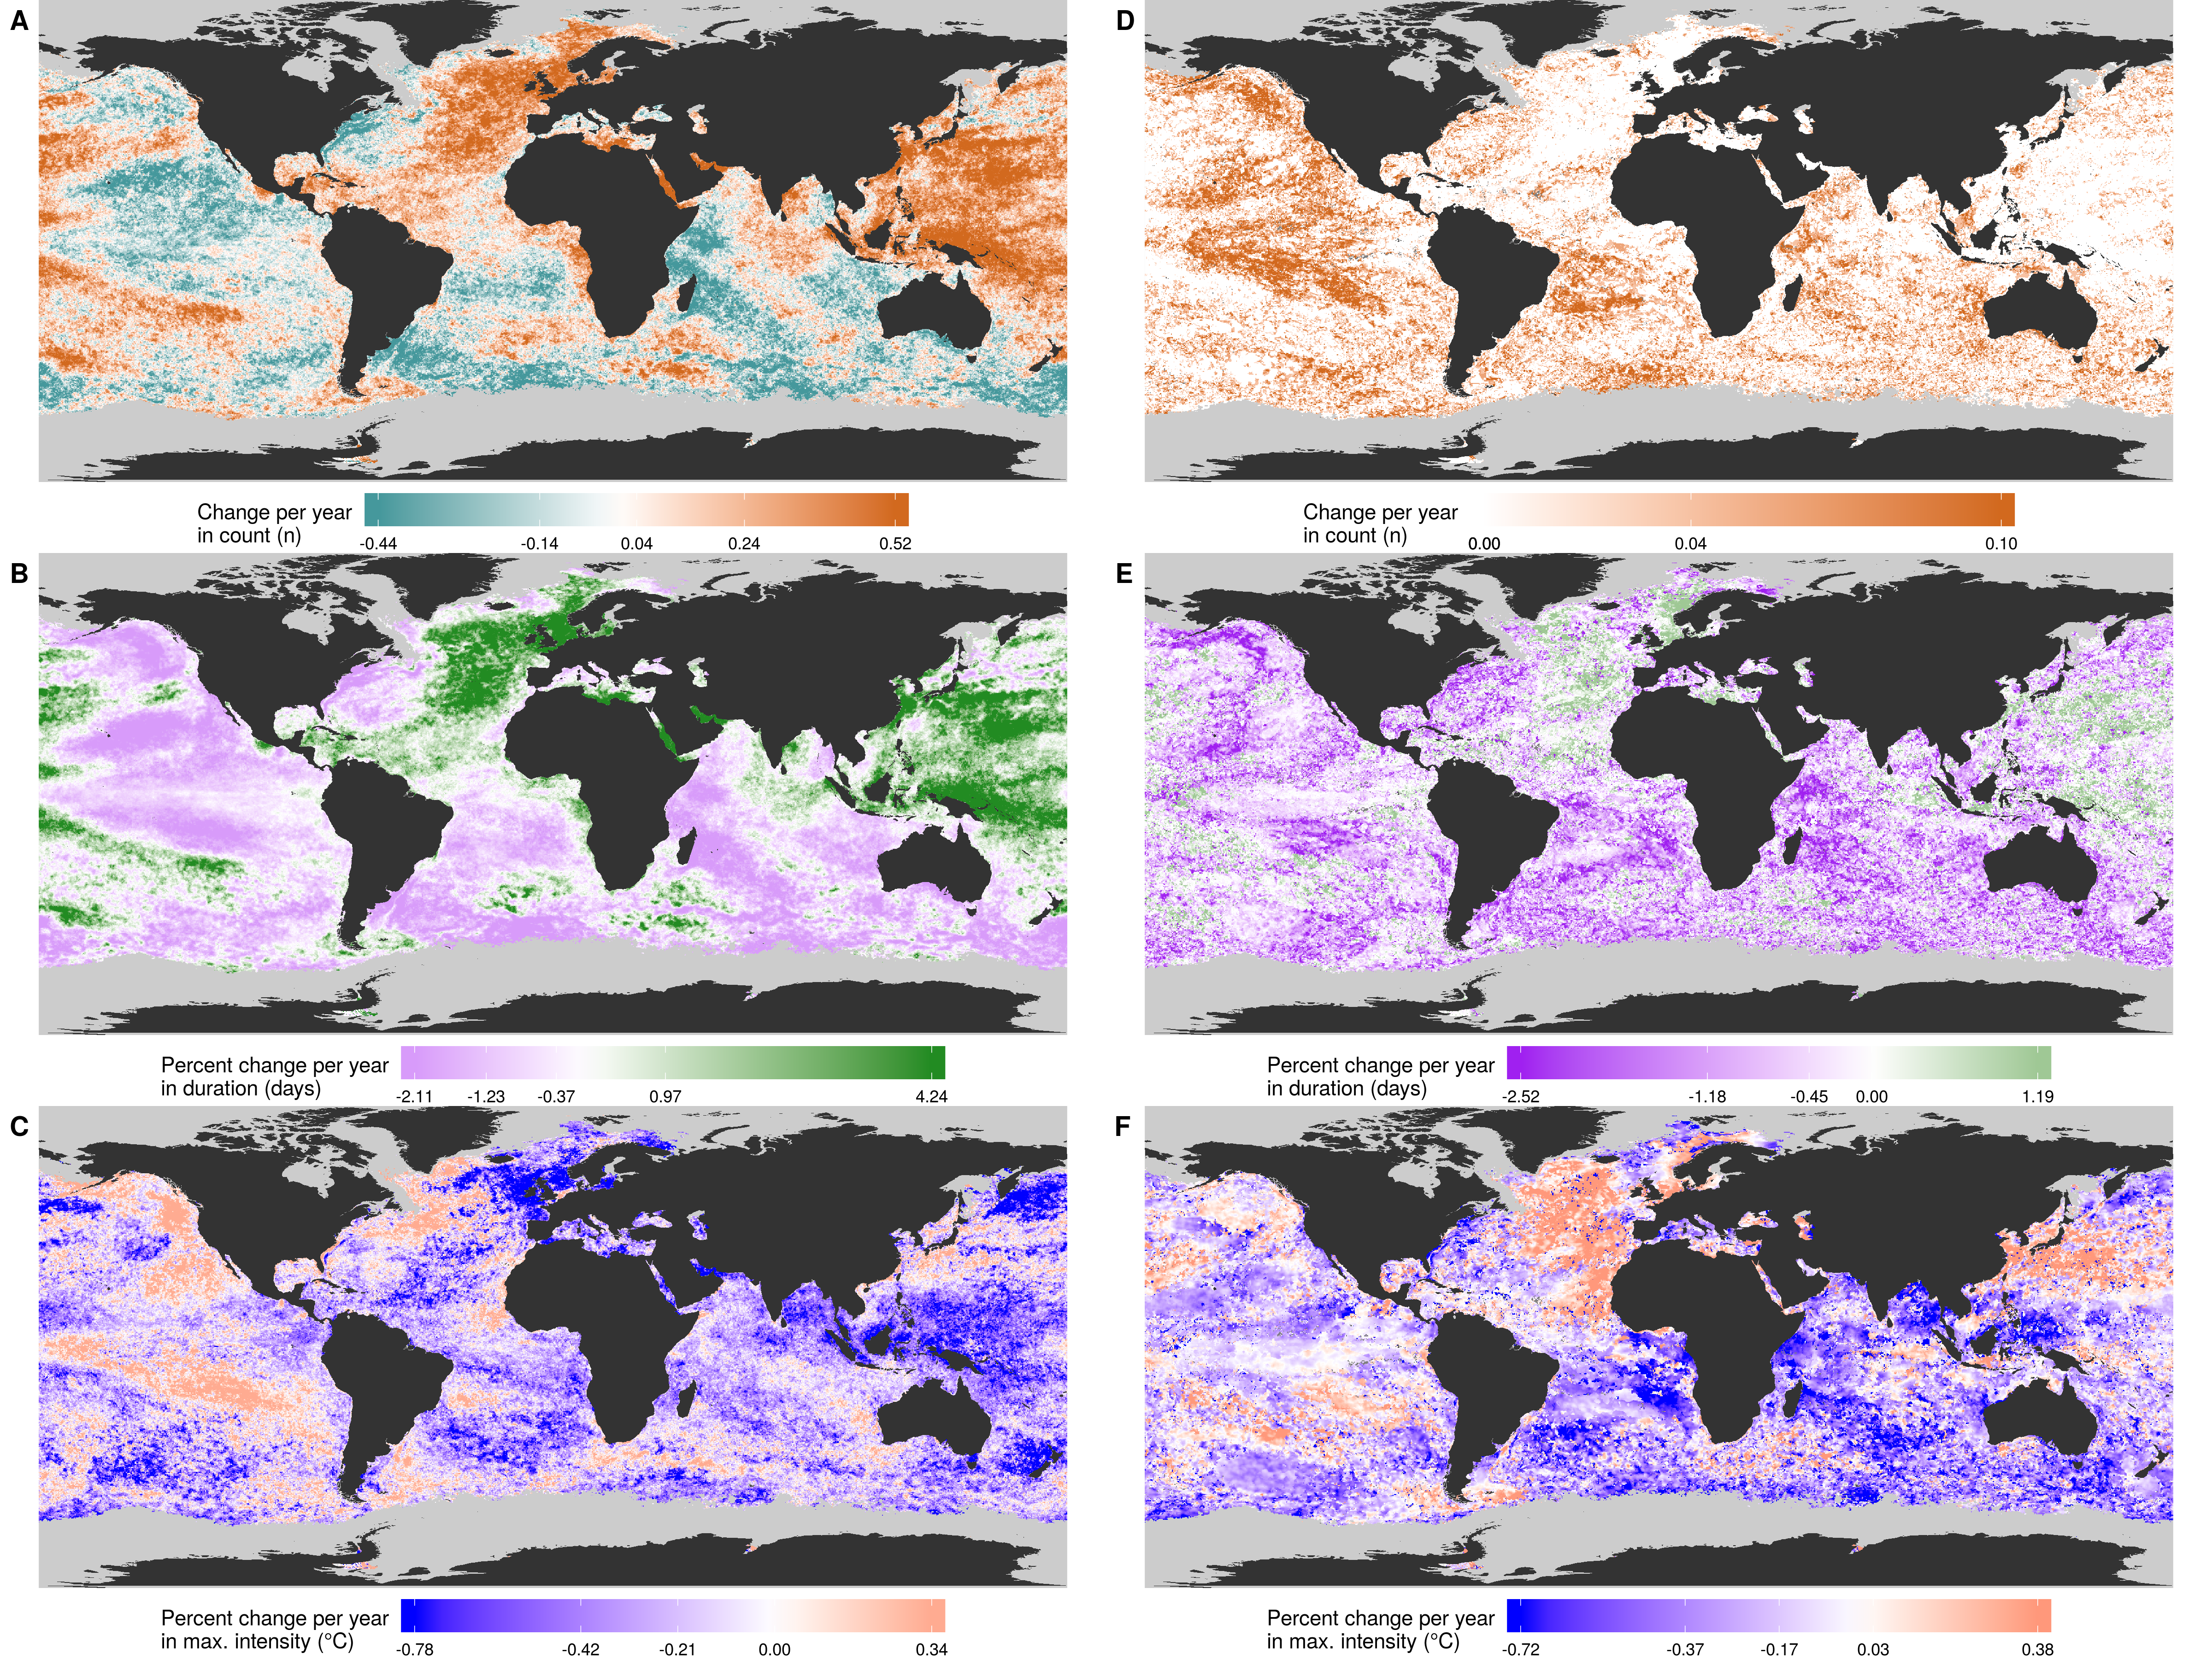
\includegraphics{../LaTeX/fig_4.png}
\caption{Figure 4: Map showing the percent increase per year in the
maximum intensity of the largest MHW detected in the most recent ten
years of data when an increasing number of years of data are used for
the calculation of the MHW.}
\end{figure}

Looking at the effect of time series length on the duration of MHWs
around the globe (Figure 5) we see a similar pattern to the effect on
maximum intensity (Figure 4). The median increase is 1.4\% per year over
the duration of the MHW detected with 10 years of data. This is not
surprising and supports the observation for maximum intensity.

\begin{figure}
\centering
\includegraphics{../LaTeX/fig_5.png}
\caption{Figure 5: Map showing the percent increase per year in the
duration of the largest MHW detected in the most recent ten years of
data when progressively more years of data are used for the calculation
of the MHW.}
\end{figure}

The fixes proposed for shorter time series may have been beneficial for
time series under 15 years in length, but the correction they provided
was not consistent. The larger issue cause by a short time series is the
amount that the centre of the climatology increases or decreases, more
so than the increase in variability caused. This is not something that
can be controlled for \emph{a-priori} and is better controlled for in a
\emph{post-hoc} manner along the same lines as the proposed fix for
decadal trends (see below).

<<<<<<< HEAD
\hypertarget{missing-data}{%
\subsection{Missing data}\label{missing-data}}
=======
\subsection{Missing data}\label{missing-data}
>>>>>>> 59f30a2abb8f68303f0eba570fc6e00bb2250a7f

The effects of missing data on the outputs of the MHW algorithm are very
pronounced. Whereas the changes in time series length may affect the
climatologies more rapidly, increases in missing data affect the MHW
metrics and the categories much more. The outputs most affected are the
threshold climatology, the duration of the MHWs, and the proportions of
MHW days in the moderate and strong categories. The maximum intensities
of the MHWs are also affected, but at 50\% missing data these did not
become significantly different from the control time series. The
proportion of severe or extreme days were not affected by missing data
as they were already so rare or non-existent. The seasonal signal was
affected very little by large proportions of missing data.

\begin{figure}
\centering
\includegraphics{../LaTeX/fig_6.png}
\caption{Figure 6: The results from Kolmogorov-Smirnov (KS) tests on the
similarity of the outputs from the MHW algorithm with optimal data
against sub-optimal time series with increasing percentages of missing
data. The climatology outputs are shown in blue, the event metrics in
green, and the category proportions in yellow-red. The solid lines show
the mean \emph{p}-value from the tests on the 100 re-sampled time series
for each step. The coloured ribbons show one standard deviation (SD) in
the \emph{p}-values for each step. The results for each reference time
series are A) Western Australia (WA), B) Northwest Atlantic (NWA), C)
Mediterranean (Med). The x-axis shows the percent of missing data in the
time series being compared against the complete (0\%; optimal) data. The
y-axis shows the range of mean \emph{p}-values from 1.0 (exact same) to
0.0 (completely different), with a horizontal dashed red line at
\emph{p}=0.05 (statistically significantly different). Any mean values
at or below the \emph{p}=0.05 line are highlighted with red squares.}
\end{figure}

The effect of random missing data on the single focus MHWs from the
three reference time series are very jagged because the missing data at
each step was only calculated once. This was done intentionally to
highlight the range that this randomness can have on the results as
compared to the changes in length (Figure 3; left column). The effect
that missing data can have on the MHW metrics depends largely on the
shape of the MHW. The WA event has a very pronounced peak (Figure 1A),
so when larger proportions of data are missing we see how likely it
becomes that this peak is not being recorded. The maximum intensity
measured in the control time series is 6.5°C, but we see that because
very few days of this MHW were so intense, increasing proportions of
missing data become more likely to remove these large values. In the NWA
event we also see a jagged effect from missing data, though less than
the WA event, this is also because of the peak in temperature for this
event. The effect on the Med event is the least pronounced. This is
because the event does not have on large peak, rather it is more even in
its exceedance above the 90th percentile threshold so missing data does
not begin to have an appreciable effect on the event until there is an
excess of 35\% of the data missing.

The duration of the MHWs are all negatively impacted by missing data,
with the longer duration MHW (WA) impacted much more than the shorter
(NWA and Med) MHWs (Figure 3; centre middle panel). Even though the
decrease in duration due to missing data is very rough, we see that it
follows a linear trend and can therefore be predicted for within a
certain range of error.

For the two shorter MHWs the increase in missing data never divides the
event up into more than two separate MHWs (Figure 3; centre top panel).
The contiguity of the WA event however is affected greatly by missing
data. With just 5\% of the data in the time series missing this event
was divided into 5 separate events. As missing data increased the count
of the divided events tended to also increase up until 27\% missing
data. At that point the event began to be divided into fewer events
again, not because they were forming back together, but rather because
there was now too little data to be detecting the splinters being formed
off of the main event.

The linear interpolation of missing data was very effective and could
potentially allow for the use of time series missing up to 50\% of their
data (Figure 7), assuming that there is not so much missing data that
there are no representative days of the MHW that one may be wanting to
study/isolate.

\begin{figure}
\centering
\includegraphics{../LaTeX/fig_7.png}
\caption{Figure 7: The same information shown in Figure 6, but with the
gaps introduced from the random missing data filled via linear
interpolation before running the MHW detection algorithm.}
\end{figure}

<<<<<<< HEAD
\hypertarget{long-term-trends}{%
\subsection{Long-term trends}\label{long-term-trends}}
=======
\subsection{Long-term trends}\label{long-term-trends}
>>>>>>> 59f30a2abb8f68303f0eba570fc6e00bb2250a7f

When adding a linear trend to the re-sampled time series we see that it
created statistically significantly different climatologies at an
exponential rate (Figure 8). The effect an added decadal trend had on
the other outputs of the MHW algorithm was roughly linear, and never
produced results significantly different from the control time series.
The maximum intensity and duration of events were affected more than the
category proportions.
<<<<<<< HEAD

\begin{figure}
\centering
\includegraphics{../LaTeX/fig_8.png}
\caption{Figure 8: The results from Kolmogorov-Smirnov (KS) tests on the
similarity of the outputs from the MHW algorithm with optimal data
against sub-optimal time series with increasingly larger linear decadal
trends added to them. The climatology outputs are shown in blue, the
event metrics in green, and the category proportions in yellow-red. The
solid lines show the mean \emph{p}-value from the tests on the 100
re-sampled time series for each step. The coloured ribbons show one
standard deviation (SD) in the \emph{p}-values for each step. The
results for each reference time series are A) Western Australia (WA), B)
Northwest Atlantic (NWA), C) Mediterranean (Med). The x-axis shows the
decadal trend added to the time series being compared against the flat
(0 added trend; optimal) data. The y-axis shows the range of mean
\emph{p}-values from 1.0 (exact same) to 0.0 (completely different),
with a horizontal dashed red line at \emph{p}=0.05 (statistically
significantly different). Any mean values at or below the \emph{p}=0.05
line are highlighted with red squares.}
\end{figure}

Adding linear long-term trends never caused the focus MHW to be
dissected into multiple events (Figure 3; top right panel). The duration
of the events are affected differently by the added linear trend. The
Med shows practically no effect, the NWA has a very slight increase with
a dramatic jump at an added trend of 0.04°C/dec, whereas the WA event
sees a massive increase due primarily to one large jump at 0.42°/dec.
The effect that the linear trend has on the maximum intensity of each
event is a simple linear function of the decadal trend and where in the
time series the event occurs. The slope for the increase in maximum
intensity for the Med MHW is more shallow than the other two because
this MHW occurred in 2003, as opposed to 2010 (WA) and 2012 (NWA).
=======

\begin{figure}
\centering
\includegraphics{../LaTeX/fig_8.png}
\caption{Figure 8: The results from Kolmogorov-Smirnov (KS) tests on the
similarity of the outputs from the MHW algorithm with optimal data
against sub-optimal time series with increasingly larger linear decadal
trends added to them. The climatology outputs are shown in blue, the
event metrics in green, and the category proportions in yellow-red. The
solid lines show the mean \emph{p}-value from the tests on the 100
re-sampled time series for each step. The coloured ribbons show one
standard deviation (SD) in the \emph{p}-values for each step. The
results for each reference time series are A) Western Australia (WA), B)
Northwest Atlantic (NWA), C) Mediterranean (Med). The x-axis shows the
decadal trend added to the time series being compared against the flat
(0 added trend; optimal) data. The y-axis shows the range of mean
\emph{p}-values from 1.0 (exact same) to 0.0 (completely different),
with a horizontal dashed red line at \emph{p}=0.05 (statistically
significantly different). Any mean values at or below the \emph{p}=0.05
line are highlighted with red squares.}
\end{figure}
>>>>>>> 59f30a2abb8f68303f0eba570fc6e00bb2250a7f

Adding linear long-term trends never caused the focus MHW to be
dissected into multiple events (Figure 3; top right panel). The duration
of the events are affected differently by the added linear trend. The
Med shows practically no effect, the NWA has a very slight increase with
a dramatic jump at an added trend of 0.04°C/dec, whereas the WA event
sees a massive increase due primarily to one large jump at 0.42°/dec.
The effect that the linear trend has on the maximum intensity of each
event is a simple linear function of the decadal trend and where in the
time series the event occurs. The slope for the increase in maximum
intensity for the Med MHW is more shallow than the other two because
this MHW occurred in 2003, as opposed to 2010 (WA) and 2012 (NWA).

\section{Discussion}\label{discussion}

An investigation into the effects that sub-optimal data have on MHW
results revealed that there are thresholds within which the outputs of
the MHW detection algorithm will remain comparable to results generated
by optimal data. Times series longer than about 15 years in length
should cause little concern regarding the reliability of the
climatologies that are derived from them. The length of a time series
has less of an effect on the other outputs of the MHW algorithm, with
lengths of 10 years not producing appreciably different outputs in MHW
metrics or category proportions. An unexpected result was that
increasing the length of a time series longer than 30 years reduced the
probability that the outputs would be comparable by as much as as
shortening the time series did. This means that the common assumptions
that using 30 years of data is the same as using \textgreater{} 30 years
of data is incorrect. In other words, the 30 year length is often
thought of as a minimum length needed to constrain the climatology but
we have shown here that using a climatology period greater than 30 years
creates different outputs. It is therefore important to stress the
adherence to the WMO standards for climatology periods as closely as
possible. Increased smoothing of the climatologies derived from
shortened time series was not an effective fix to the other outputs of
the MHW algorithm. In the global analysis we did see that there is a
relationship between decadal trend in seawater temperature and the
increase in the duration and maximum intensity of events detected within
the most recent decade of data. This can be used to infer a likely
correction for the resultant MHW metrics.

The MHW algorithm proved to be resilient to missing data and so long as
one does not have particularly large gaps (e.g.~greater than a week at a
time), time series missing as much as 20\% of their data may be used
without concern. Greater amounts of missing data could still be used
with some caution as the outputs of the MHW algorithm did not differ
significantly on average when as much as 50\% missing data were present.
It is not however recommended to consider the outputs of time series
with this much missing data to be comparable to outputs from an optimal
time series. This is because the number of events detected in the time
series with high amounts will differ greatly. The overall metrics of the
events may be comparable between the time series, but the actual events
detected will be different. A simple correction for missing data in a
time series is to linearly interpolate over the gaps. It is not however
recommended to do this with more than 40\% missing data as this begins
to dramatically distort the algorithms ability to compute metrics for
individual MHWs. If this is necessary to do for some reason, the
resultant MHWs for the entire time series can be used to infer the
chronic and acute stress that organisms may face in a given location,
but any individual events detected should not be taken as an accurate
recording.

The decadal trends in times series very rapidly affect the creation of
climatologies. That being said, normal ranges of decadal trends
(e.g.~0.1 -- 0.5C/dec) do not have a significant effect on the detection
of MHW metrics. Furthermore, the effect of decadal trends is very
predictable and when taken with time series length and the year in which
an event in question has occurred it is possible to infer a correction
for the maximum intensity. The effect this has on the duration can also
be worked out by considering the general raise (or fall) in the mean
climatology and how that may engulf neighbouring days or even other
events. A concept to consider with the increase in duration from added
decadal trends is that the temperatures in the time series increase
``faster'' than the 90th percentile threshold. So as the decadal trend
increases, the MHW effectively spreads outwards. If the rate of
onset/decline for the MHW was more gradual (e.g.~the NWA event) it will
increase in duration more rapidly. If the rate of onset/decline was more
rapid (e.g.~the Med event), then the duration of the MHW won't change
much with a larger decadal trend. If MHWs have close neighbours then as
they spread outward they may encounter and be engulfed into one another.
This reduces the overall count of the MHWs detected in a time series
while increasing the apparent duration of the events.

<<<<<<< HEAD
\hypertarget{conclusions}{%
\section{Conclusions}\label{conclusions}}
=======
\section{Conclusions}\label{conclusions}
>>>>>>> 59f30a2abb8f68303f0eba570fc6e00bb2250a7f

We have shown here that researchers must not shy away from the use of
sub-optimal time series when the situation calls for it, such as coastal
research or sub-surface analyses. Time series length may have an
unpredictable effect on MHW results, but this may be corrected for
within reason, and we have shown that time series lengths as short as 10
years are still useful for MHW research. Any shorter than 10 years
however and the relationship between time series length and the effect
on MHW metrics becomes too unpredictable to provide any corrections with
confidence. Missing data has a larger effect, but is less of a concern
as linear interpolation can largely fix the challenges this creates, up
to a threshold of 40\% missing data. Lastly, the errors introduced by
long-term trends in the data are the most predictable and when taken
with time series length may be corrected for as well. The MHW detection
algorithm is very robust and we have shown here that one may be
confident in the inter-comparability of ones results when using time
series within a generous range of sub-optimal data challenges.

\section*{References}\label{references}
\addcontentsline{toc}{section}{References}

\hypertarget{refs}{}
\hypertarget{ref-Baumgartner1992}{}
Baumgartner, TR. 1992. ``Reconstruction of the History of the Pacific
Sardine and Northern Anchovy Populations over the Past Two Millenia from
Sediments of the Santa Barbara Basin, California.'' \emph{CalCOFI Rep}
33: 24--40.

\hypertarget{ref-Hobday2016}{}
Hobday, Alistair J, Lisa V Alexander, Sarah E Perkins, Dan A Smale,
Sandra C Straub, Eric CJ Oliver, Jessica A Benthuysen, et al. 2016. ``A
Hierarchical Approach to Defining Marine Heatwaves.'' \emph{Progress in
Oceanography} 141. Elsevier: 227--38.

\hypertarget{ref-Hobday2018}{}
Hobday, Alistair J, Eric CJ Oliver, Alex Sen Gupta, Jessica A
Benthuysen, Michael T Burrows, Markus G Donat, Neil J Holbrook, et al.
2018. ``Categorizing and Naming Marine Heatwaves.'' \emph{Oceanography}
31 (2). JSTOR: 162--73.

\hypertarget{ref-Oliver2018}{}
Oliver, Eric CJ, Markus G Donat, Michael T Burrows, Pippa J Moore, Dan A
Smale, Lisa V Alexander, Jessica A Benthuysen, et al. 2018. ``Longer and
More Frequent Marine Heatwaves over the Past Century.'' \emph{Nature
Communications} 9 (1). Nature Publishing Group: 1324.

\hypertarget{ref-WMO2011}{}
Organization, World Meteorological. 2011. \emph{Guide to Climatological
Practices}. World Meteorological Organization (WMO).

\hypertarget{ref-WMO2017}{}
---------. 2017. \emph{WMO Guidelines on the Calculation of Climate
Normals}. World Meteorological Organization (WMO).

\hypertarget{ref-IPCC2014}{}
Pachauri, Rajendra K, Leo Meyer, J van Ypersele, Sander Brinkman, Line
van Kesteren, Noëmie Leprince-Ringuet, and Fijke Van Boxmeer. 2014.
``Climate Change 2014 Synthesis Report.''

\hypertarget{ref-Philander1983}{}
Philander, S George H. 1983. ``El Nino Southern Oscillation Phenomena.''
\emph{Nature} 302 (5906). Nature Publishing Group: 295.

\hypertarget{ref-Reynolds2007}{}
Reynolds, Richard W, Thomas M Smith, Chunying Liu, Dudley B Chelton,
Kenneth S Casey, and Michael G Schlax. 2007. ``Daily
high-resolution-blended analyses for sea surface temperature.''
\emph{Journal of Climate} 20 (22). NOAA, Natl Climatic Data Ctr,
Asheville, NC 28801 USA: 5473--96.

\hypertarget{ref-Salinger2016}{}
Salinger, J., A.J. Hobday, R.J. Matear, T.J. O'Kane, J.S. Risbey, P.
Dunstan, J.P. Eveson, et al. 2016. ``Chapter One - Decadal-Scale
Forecasting of Climate Drivers for Marine Applications.'' In, edited by
Barbara E. Curry, 74:1--68. Advances in Marine Biology. Academic Press.
doi:\href{https://doi.org/https://doi.org/10.1016/bs.amb.2016.04.002}{https://doi.org/10.1016/bs.amb.2016.04.002}.

\hypertarget{ref-Schlegel2018}{}
Schlegel, Robert W, and Albertus J Smit. 2018. ``HeatwaveR: A Central
Algorithm for the Detection of Heatwaves and Cold-Spells.'' \emph{The
Journal of Open Source Software} 3: 821.

\hypertarget{ref-Smale2019}{}
Smale, Dan A, Thomas Wernberg, Eric CJ Oliver, Mads Thomsen, Ben P
Harvey, Sandra C Straub, Michael T Burrows, et al. 2019. ``Marine
Heatwaves Threaten Global Biodiversity and the Provision of Ecosystem
Services.'' \emph{Nature Climate Change}. Nature Publishing Group, 1.

<<<<<<< HEAD
\leavevmode\hypertarget{ref-Wasserstein2019}{}%
Wasserstein, Ronald L., Allen L. Schirm, and Nicole A. Lazar. 2019.
``Moving to a World Beyond `P\textless{}0.05'.'' \emph{The American
Statistician} 73 (sup1). Taylor \& Francis: 1--19.
\url{https://doi.org/10.1080/00031305.2019.1583913}.

\leavevmode\hypertarget{ref-Zhao2019}{}%
=======
\hypertarget{ref-Wasserstein2019}{}
Wasserstein, Ronald L., Allen L. Schirm, and Nicole A. Lazar. 2019.
``Moving to a World Beyond `P\textless{}0.05'.'' \emph{The American
Statistician} 73 (sup1). Taylor \& Francis: 1--19.
doi:\href{https://doi.org/10.1080/00031305.2019.1583913}{10.1080/00031305.2019.1583913}.

\hypertarget{ref-Zhao2019}{}
>>>>>>> 59f30a2abb8f68303f0eba570fc6e00bb2250a7f
Zhao, Zijie, and Maxime Marin. 2019. ``A Matlab Toolbox to Detect and
Analyze Marine Heatwaves.'' \emph{The Journal of Open Source Software}
4: 1124.


\end{document}
